\documentclass{standalone}
\usepackage{tikz}
\usetikzlibrary{patterns, positioning}
\usepackage[sfdefault]{ClearSans} %% option 'sfdefault' activates Clear Sans as the default text font
\usepackage[T1]{fontenc}

\begin{document}
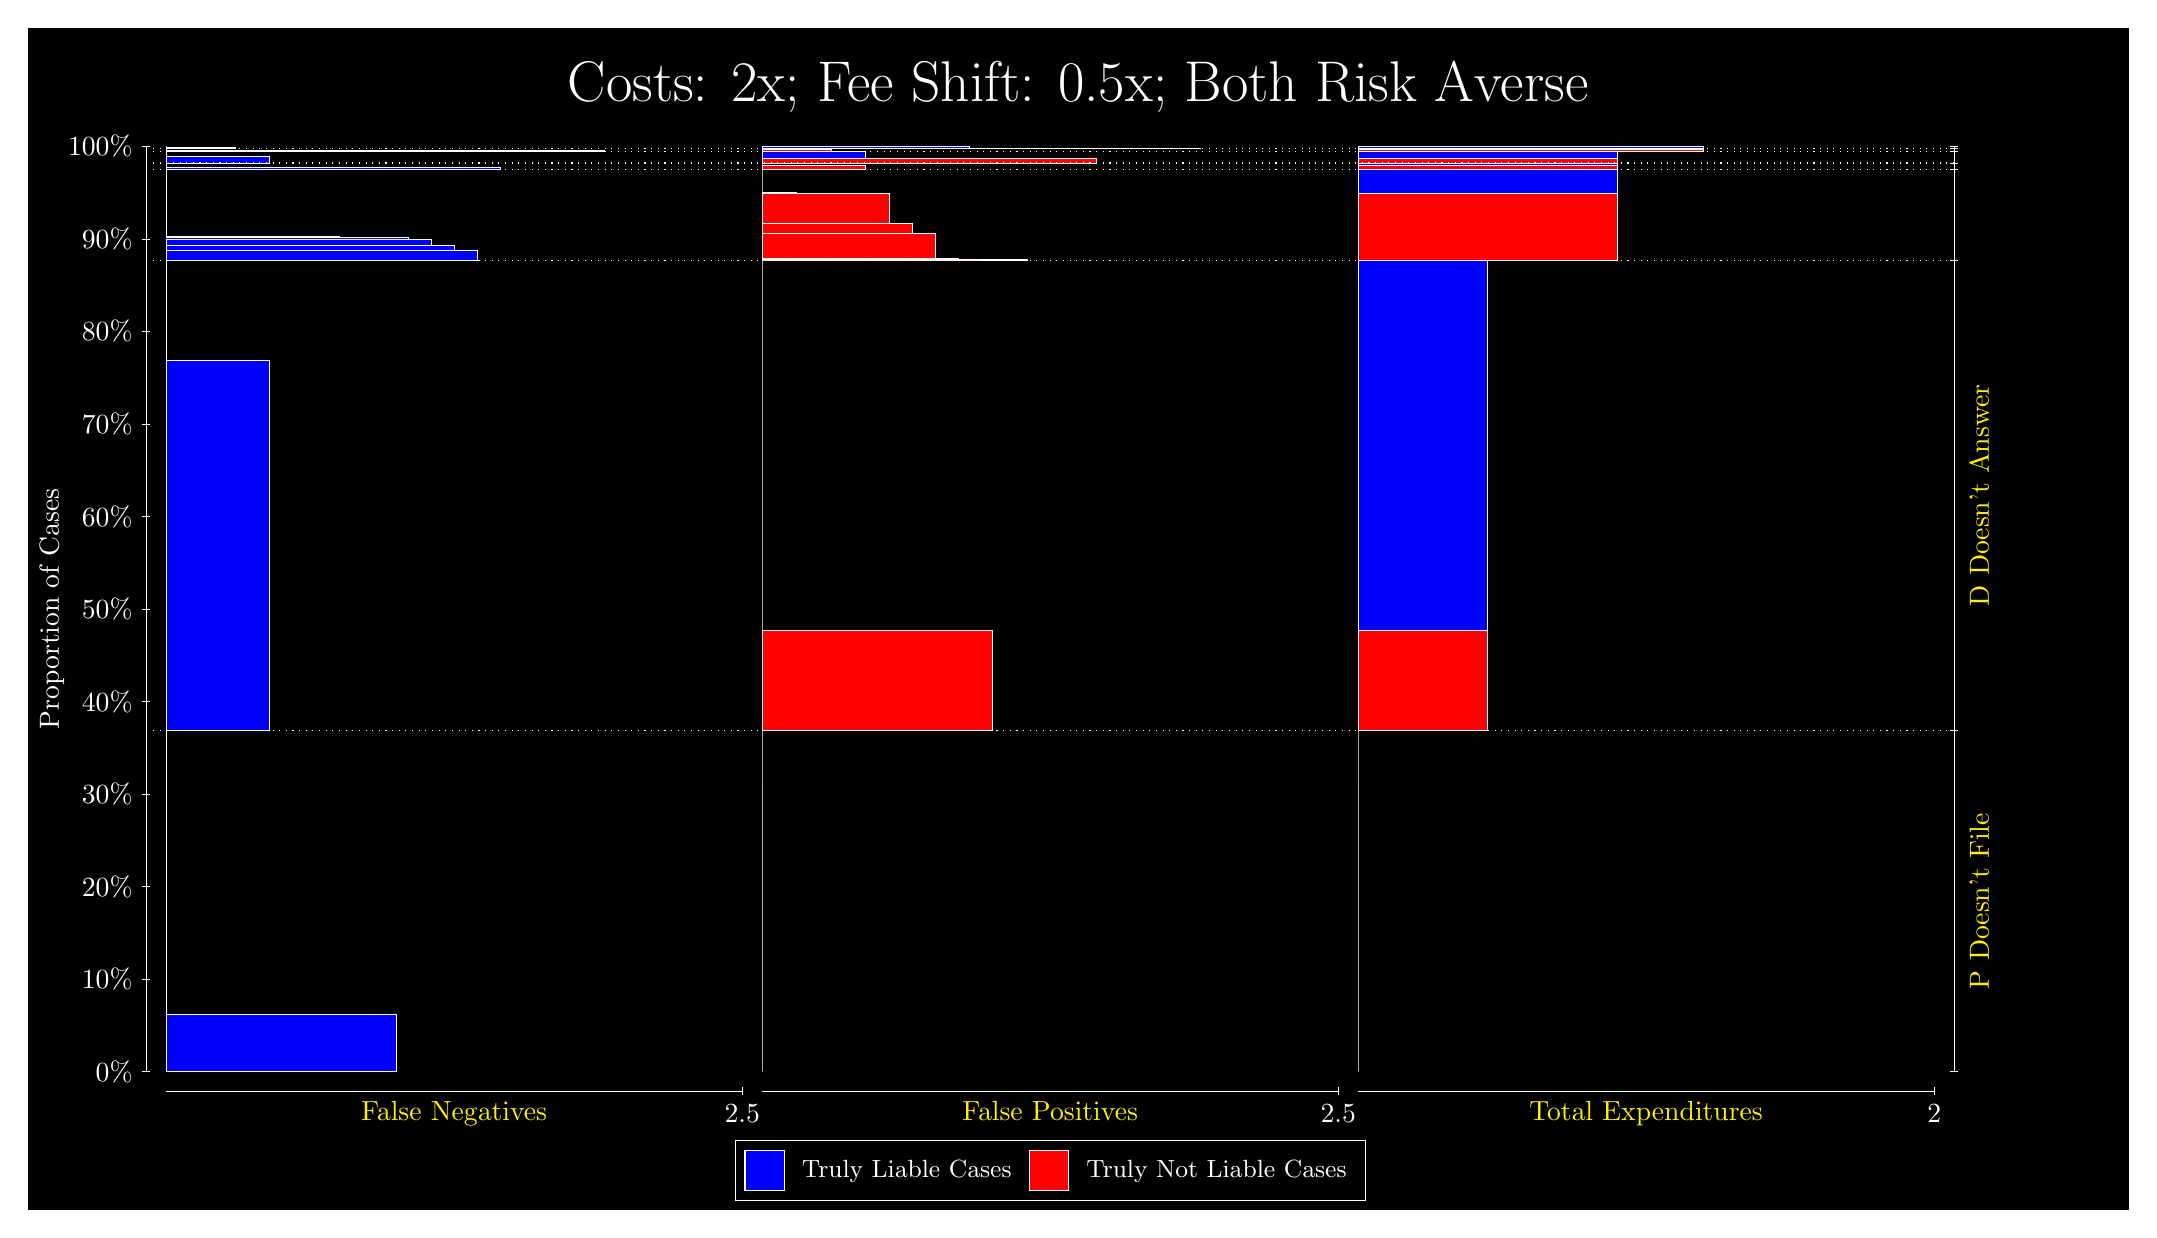
\begin{tikzpicture}
\draw[fill=black] (0,0) rectangle (26.667,15);
\draw[text=white] (0,13.5) rectangle (26.667,15) node[midway] {\huge Costs: 2x; Fee Shift: 0.5x; Both Risk Averse};
\draw[white, very thin] (1.5,1.75) -- (1.5,13.5);
\node[rotate=90, text=white, anchor=center] at (0.3, 7.625) {Proportion of Cases};
\draw[white, very thin] (1.45,1.75) -- (1.55,1.75);
\node[text=white, anchor=east] at (1.45, 1.75) {0\%};
\draw[white, very thin] (1.45,2.925) -- (1.55,2.925);
\node[text=white, anchor=east] at (1.45, 2.925) {10\%};
\draw[white, very thin] (1.45,4.1) -- (1.55,4.1);
\node[text=white, anchor=east] at (1.45, 4.1) {20\%};
\draw[white, very thin] (1.45,5.275) -- (1.55,5.275);
\node[text=white, anchor=east] at (1.45, 5.275) {30\%};
\draw[white, very thin] (1.45,6.45) -- (1.55,6.45);
\node[text=white, anchor=east] at (1.45, 6.45) {40\%};
\draw[white, very thin] (1.45,7.625) -- (1.55,7.625);
\node[text=white, anchor=east] at (1.45, 7.625) {50\%};
\draw[white, very thin] (1.45,8.8) -- (1.55,8.8);
\node[text=white, anchor=east] at (1.45, 8.8) {60\%};
\draw[white, very thin] (1.45,9.975) -- (1.55,9.975);
\node[text=white, anchor=east] at (1.45, 9.975) {70\%};
\draw[white, very thin] (1.45,11.15) -- (1.55,11.15);
\node[text=white, anchor=east] at (1.45, 11.15) {80\%};
\draw[white, very thin] (1.45,12.325) -- (1.55,12.325);
\node[text=white, anchor=east] at (1.45, 12.325) {90\%};
\draw[white, very thin] (1.45,13.5) -- (1.55,13.5);
\node[text=white, anchor=east] at (1.45, 13.5) {100\%};

\draw[white, very thin] (24.457,1.75) -- (24.457,13.5);
\draw[white, very thin] (24.407,1.75) -- (24.507,1.75);
\node[anchor=west] at (24.407, 1.75) {};
\draw[white, very thin] (24.407,6.0782) -- (24.507,6.0782);
\node[anchor=west] at (24.407, 6.0782) {};
\draw[white, very thin] (24.407,12.055) -- (24.507,12.055);
\node[anchor=west] at (24.407, 12.055) {};
\draw[white, very thin] (24.407,13.205) -- (24.507,13.205);
\node[anchor=west] at (24.407, 13.205) {};
\draw[white, very thin] (24.407,13.288) -- (24.507,13.288);
\node[anchor=west] at (24.407, 13.288) {};
\draw[white, very thin] (24.407,13.432) -- (24.507,13.432);
\node[anchor=west] at (24.407, 13.432) {};
\draw[white, very thin] (24.407,13.469) -- (24.507,13.469);
\node[anchor=west] at (24.407, 13.469) {};
\draw[white, very thin] (24.407,13.5) -- (24.507,13.5);
\node[anchor=west] at (24.407, 13.5) {};

\draw[white, very thin, fill=blue] (1.75,1.75) rectangle (4.6775,2.475);
\draw[white, very thin, fill=red] (1.75,2.475) rectangle (1.75,6.0782);
\draw[white, very thin, fill=blue] (1.75,6.0782) rectangle (3.0674,10.777);
\draw[white, very thin, fill=red] (1.75,10.777) rectangle (1.75,12.055);
\draw[white, very thin, fill=blue] (1.75,12.055) rectangle (5.7022,12.177);
\draw[white, very thin, fill=blue] (1.75,12.177) rectangle (5.4094,12.238);
\draw[white, very thin, fill=blue] (1.75,12.238) rectangle (5.1167,12.32);
\draw[white, very thin, fill=blue] (1.75,12.32) rectangle (4.8239,12.339);
\draw[white, very thin, fill=blue] (1.75,12.339) rectangle (4.5312,12.34);
\draw[white, very thin, fill=blue] (1.75,12.34) rectangle (3.9457,12.359);
\draw[white, very thin, fill=red] (1.75,12.359) rectangle (1.75,13.205);
\draw[white, very thin, fill=blue] (1.75,13.205) rectangle (5.9949,13.239);
\draw[white, very thin, fill=red] (1.75,13.239) rectangle (1.75,13.288);
\draw[white, very thin, fill=blue] (1.75,13.288) rectangle (3.0674,13.37);
\draw[white, very thin, fill=red] (1.75,13.37) rectangle (1.75,13.432);
\draw[white, very thin, fill=blue] (1.75,13.432) rectangle (7.3123,13.444);
\draw[white, very thin, fill=red] (1.75,13.444) rectangle (1.75,13.469);
\draw[white, very thin, fill=blue] (1.75,13.469) rectangle (2.6283,13.489);
\draw[white, very thin, fill=red] (1.75,13.489) rectangle (1.75,13.5);
\draw[white, very thin, fill=red] (9.3189,1.75) rectangle (9.3189,5.3532);
\draw[white, very thin, fill=blue] (9.3189,5.3532) rectangle (9.3189,6.0782);
\draw[white, very thin, fill=red] (9.3189,6.0782) rectangle (12.246,7.356);
\draw[white, very thin, fill=blue] (9.3189,7.356) rectangle (9.3189,12.055);
\draw[white, very thin, fill=red] (9.3189,12.055) rectangle (12.686,12.062);
\draw[white, very thin, fill=red] (9.3189,12.062) rectangle (12.1,12.062);
\draw[white, very thin, fill=red] (9.3189,12.062) rectangle (11.807,12.082);
\draw[white, very thin, fill=red] (9.3189,12.082) rectangle (11.515,12.391);
\draw[white, very thin, fill=red] (9.3189,12.391) rectangle (11.222,12.524);
\draw[white, very thin, fill=red] (9.3189,12.524) rectangle (10.929,12.9);
\draw[white, very thin, fill=blue] (9.3189,12.9) rectangle (9.758,12.92);
\draw[white, very thin, fill=blue] (9.3189,12.92) rectangle (9.3189,13.205);
\draw[white, very thin, fill=red] (9.3189,13.205) rectangle (10.636,13.254);
\draw[white, very thin, fill=blue] (9.3189,13.254) rectangle (9.3189,13.288);
\draw[white, very thin, fill=red] (9.3189,13.288) rectangle (13.564,13.35);
\draw[white, very thin, fill=blue] (9.3189,13.35) rectangle (10.636,13.432);
\draw[white, very thin, fill=red] (9.3189,13.432) rectangle (10.197,13.458);
\draw[white, very thin, fill=blue] (9.3189,13.458) rectangle (9.3189,13.469);
\draw[white, very thin, fill=red] (9.3189,13.469) rectangle (14.881,13.481);
\draw[white, very thin, fill=blue] (9.3189,13.481) rectangle (11.954,13.5);
\draw[white, very thin, fill=red] (16.888,1.75) rectangle (16.888,5.3532);
\draw[white, very thin, fill=blue] (16.888,5.3532) rectangle (16.888,6.0782);
\draw[white, very thin, fill=red] (16.888,6.0782) rectangle (18.534,7.356);
\draw[white, very thin, fill=blue] (16.888,7.356) rectangle (18.534,12.055);
\draw[white, very thin, fill=red] (16.888,12.055) rectangle (20.181,12.9);
\draw[white, very thin, fill=blue] (16.888,12.9) rectangle (20.181,13.205);
\draw[white, very thin, fill=red] (16.888,13.205) rectangle (20.181,13.254);
\draw[white, very thin, fill=blue] (16.888,13.254) rectangle (20.181,13.288);
\draw[white, very thin, fill=red] (16.888,13.288) rectangle (20.181,13.35);
\draw[white, very thin, fill=blue] (16.888,13.35) rectangle (20.181,13.432);
\draw[white, very thin, fill=red] (16.888,13.432) rectangle (21.279,13.458);
\draw[white, very thin, fill=blue] (16.888,13.458) rectangle (21.279,13.469);
\draw[white, very thin, fill=red] (16.888,13.469) rectangle (21.279,13.481);
\draw[white, very thin, fill=blue] (16.888,13.481) rectangle (21.279,13.5);
\draw[white, dotted] (1.5,6.0782) -- (24.457,6.0782);
\draw[white, dotted] (1.5,12.055) -- (24.457,12.055);
\draw[white, dotted] (1.5,13.205) -- (24.457,13.205);
\draw[white, dotted] (1.5,13.288) -- (24.457,13.288);
\draw[white, dotted] (1.5,13.432) -- (24.457,13.432);
\draw[white, dotted] (1.5,13.469) -- (24.457,13.469);
\draw[white, very thin] (1.75,1.5) -- (9.0689,1.5);
\node[text=yellow, anchor=north] at (5.4094, 1.5) {False Negatives};
\draw[white, very thin] (9.0689,1.45) -- (9.0689,1.55);
\node[text=white, anchor=north] at (9.0689, 1.45) {2.5};

\draw[white, very thin] (9.3189,1.5) -- (16.638,1.5);
\node[text=yellow, anchor=north] at (12.978, 1.5) {False Positives};
\draw[white, very thin] (16.638,1.45) -- (16.638,1.55);
\node[text=white, anchor=north] at (16.638, 1.45) {2.5};

\draw[white, very thin] (16.888,1.5) -- (24.207,1.5);
\node[text=yellow, anchor=north] at (20.547, 1.5) {Total Expenditures};
\draw[white, very thin] (24.207,1.45) -- (24.207,1.55);
\node[text=white, anchor=north] at (24.207, 1.45) {2};

\node[text=yellow, centered, rotate=90] at (24.777, 3.9141) {P Doesn't File};
\node[text=yellow, centered, rotate=90] at (24.777, 9.0664) {D Doesn't Answer};






\draw (12.978300999999998,1.5) node[draw=none] (baseCoordinate) {};
\begin{scope}[align=center]
        \matrix[scale=0.5, draw=white, below=0.5cm of baseCoordinate, nodes={draw}, column sep=0.1cm]{
            \node[rectangle, draw, minimum width=0.5cm, minimum height=0.5cm, fill=blue] {}; &
            \node[draw=none, font=\small, text=white] (B) {Truly Liable Cases}; &
            \node[rectangle, draw, minimum width=0.5cm, minimum height=0.5cm, fill=red] {}; &
            \node[draw=none, font=\small, text=white] (B) {Truly Not Liable Cases}; \\
            };
\end{scope}

\end{tikzpicture}
\end{document}